\def\CTeXPreproc{Created by ctex v0.2.9, don't edit!}
%\documentclass{beamer}
\documentclass[%handout,
xcolor=pdftex]{beamer}
\mode<presentation> {
  \usetheme{Warsaw}
  \setbeamercovered{transparent}
}
\let\Tiny=\tiny
\usetheme{Singapore}
\usecolortheme{dolphin}
\usepackage{amsmath}
\usepackage{textcomp}
\usepackage{amssymb}
\usepackage{amsthm}
\usepackage{graphicx}
\usepackage{color}
\usepackage{lipsum}
\usepackage{hyperref}
\usepackage{multirow}
\usepackage{bm}
\DeclareMathSymbol{\Phi}{\mathalpha}{operators}{8}
%\setbeamertemplate{headline}{}
\setbeamertemplate{footline}[page number]
\newcommand\Fontvi{\fontsize{9pt}{8}\selectfont}
\newcommand\Fontvii{\fontsize{7pt}{8}\selectfont}
\newcommand{\backupbegin}{
   \newcounter{finalframe}
   \setcounter{finalframe}{\value{framenumber}}
}
\newcommand{\backupend}{
   \setcounter{framenumber}{\value{finalframe}}
}\newtheorem{proposition}{Proposition}
\title{Unit 16: Seasonal ARIMA Models}
\author[STAT 5170: Applied Time Series, Unit 16]{Jeffrey Woo}
\institute{Department of Statistics, University of Virginia}
\date{Spring 2020}

\AtBeginSubsection[] {
  \begin{frame}<beamer>{Outline}
    \tableofcontents[currentsection,currentsubsection]
  \end{frame}
}



\begin{document}


\frame{\titlepage}


\begin{frame}
\frametitle{Readings for Unit 16}

Textbook chapter 3.9 (from page 149 after example 3.47).

\end{frame}



\begin{frame}
\frametitle{Last Unit}
\begin{enumerate}
\item ACF, PACF for seasonal ARMA models.
\item Multiplicative Seasonal ARMA Models.
\end{enumerate}
\end{frame}

\begin{frame}
\frametitle{This Unit}

\begin{enumerate}
\item SARIMA models to account for non-seasonal and seasonal differencing.
\item Building SARIMA models.
\end{enumerate}


\end{frame}


\begin{frame}
\frametitle{Motivation}

In Unit 15, we looked at the pure seasonal ARMA model, and the multiplicative seasonal ARMA model. These models assumed stationarity. In this unit, we consider non-stationarity and apply differencing to the non-seasonal and seasonal components.

\end{frame}

\section{Seasonal Trend}
\frame{\tableofcontents[currentsection]}

\begin{frame}
\frametitle{Seasonal Trend}

Consider the following time series:
$$
x_t=S_t+ y_t
$$
where $y_t$ is stationary and $S_t$ is a seasonal trend.

\end{frame}

\begin{frame}
\frametitle{Seasonal Trend}
Since $S_t$ is a seasonal trend, we have
$$
S_t=S_{t-s}=S_{t+s}
$$
where $s$ is the length of the period. For example, for monthly
data, a reasonable choice of $s$ is 12. For quarterly data,
$s=4$. 

Consider
$$
S_t=cos(2 \pi \frac{t}{s}).
$$
Then $S_t$ is a periodic function with period $s$. How can we get rid of this trend?  In the past, we've done  a
number of things namely regression, smoothing, and
differencing.

\end{frame}

\begin{frame}
\frametitle{Seasonal Trend}

We usually apply seasonal differencing, where we difference across the period.

\begin{eqnarray*}
(1-B^s)x_t &=& \nonumber \\
           &=& \nonumber \\
           &=& \nonumber \\
           &=& 
\end{eqnarray*}
If $s=12$, then we have a stationary MA$(1)_{12}$.

\end{frame}

\begin{frame}
\frametitle{Seasonal Trend}

In general, we need seasonal differencing when the ACF of the time series \underline{\hspace{55 mm}}. We can represent the differencing using the following notation
$$
\nabla_s^D=(1-B^s)^D.
$$

Typically, $D=1$ is sufficient to obtain seasonal stationarity. %Seasonal differencing can also remove a seasonal \underline{\hspace{20 mm}}.

\end{frame}

\section{SARIMA Model}
\frame{\tableofcontents[currentsection]}

\begin{frame}
\frametitle{SARIMA Model}

In many settings with seasonal data, \underline{\hspace{25 mm}} components may contribute to the model. For example, in monthly sales of ice cream, sales in the previous month (or two), together with sales from the same month a year ago, may help predict future sales.

\end{frame}


\begin{frame}
\frametitle{SARIMA Model}

If a linear trend is also present in the data (along with seasonality), we will probably also need a non-seasonal difference. Therefore, a non-seasonal and seasonal difference will be applied. We end up analyzing

$$
(1-B^{12})(1-B)x_t =
$$

\end{frame}


\begin{frame}
\frametitle{SARIMA Model}

This type of differencing leads us to the definition of the full SARIMA model which we denote by
$$
{\rm ARIMA}(p,d,q) \times (P,D,Q)_s
$$
and the model is
\begin{equation}
\Phi_{P}(B^s) \phi(B) \nabla_s^D \nabla^d x_t=\alpha + \Theta_{Q}(B^s) \theta(B) w_t,
\end{equation}

\end{frame}

\begin{frame}
\frametitle{SARIMA Model}

where
\begin{eqnarray*}
\phi(B) &=& 1-\phi_1 B - \phi_2 B^2 -\cdots - \phi_p B^p\\
\theta(B) &=& 1+\theta_1 B +\theta_2 B^2 +\cdots + \theta_q B^q\\
\Phi_{P}(B^s) &=& 1-\Phi_1 B^s - \Phi_2 B^{2s} - \cdots - \Phi_P B^{Ps}\\
\Theta_{Q}(B^s) &=& 1+\Theta_1 B^s+\Theta_2 B^{2s} +\cdots +\Theta_Q B^{Qs}\\
\nabla^d x_t &=&(1-B)^d x_{t}, \quad \nabla_s^D  x_t = (1-B^s)^Dx_t\\
\alpha &=& \mu(1 - \phi_1 - \cdots \phi_p)(1 - \Phi_1 - \cdots - \Phi_P)
\end{eqnarray*}

\end{frame}

\begin{frame}
\frametitle{SARIMA Model}

\textbf{Question}: How do we write an ARIMA$(0,1,1) \times (0,1,1)_{4}$ model?

\vspace{50mm}

\end{frame}




\begin{frame}
\frametitle{SARIMA Model}

The rest of the analysis is very similar to what we did
for the regular ARIMA models.  We will use plotting including
ACF and PACF to help discover $s$ and also the amount of
differencing that is necessary.  Then we will attempt to fit
appropriate models using AIC and parameter estimates to guide
us.  We will use the same diagnostics to evaluate the
appropriateness of the fits.

\end{frame}

\section{Building SARIMA Models}
\frame{\tableofcontents[currentsection]}

\begin{frame}
\frametitle{Building SARIMA Models}

Just like how we built ARIMA models in unit 14, the main steps in building SARIMA models consist of the following:

\begin{itemize}
\item Exploratory data analysis.
\item Model estimation.
\item Model diagnostics.
\item Model selection.
\end{itemize}


\end{frame}


\begin{frame}
\frametitle{Exploratory Data Analysis}

We typically look at

\begin{itemize}
\item the time series plot,
\item the ACF,
\item and the PACF
\end{itemize}

of the data. This step guides us to our choice for the elements of the SARIMA model, $p,d,q, P, D, Q, s$.


\end{frame}

\begin{frame}
\frametitle{Exploratory Data Analysis: Time Series Plot}

With the time series plot, we examine for trend and seasonality. Typically, understanding what the data describes will help us know what the period is, and what lags to look out for, so you should have an idea of what value $s$ is.


\end{frame}

\begin{frame}
\frametitle{Exploratory Data Analysis: Differencing}

The general guidelines for differencing are:

\begin{itemize}
\item Seasonality and no trend: Take a difference of lag $s$.
\item Linear trend and no seasonality: Take first difference like with ARIMA model. If quadratic trend and no seasonality, take second difference.
\item Seasonality and trend: Apply non-seasonal and seasonal differences, as successive operations in either order.
\end{itemize}

Based on these, you should have an idea of what $d$ and $D$ are.

\end{frame}

\begin{frame}
\frametitle{Exploratory Data Analysis: ACF and PACF}

Examine the ACF and PACF of the differenced data. Some guidelines:

\begin{itemize}
\item Non-seasonal terms: Examine the early lags $(1, 2, 3, \cdots)$ to judge the values of $p$ and $q$. This will be similar to what was done with ARIMA models (Unit 14).
\item Seasonal terms: Examine the pattern of the lags that are multiples of $s$. Typically you should look at the first two or three multiples. Judge the values of $P$ and $Q$ as in slide 23 from Unit 15.
\end{itemize}

\end{frame}

\begin{frame}
\frametitle{Model Estimation}

After exploratory data analysis, you should have an idea (or ideas) about the values of $p, d, q, P, D, Q, s$. When using R, I highly suggest using the original data, and then specify the values of the differencing used.

\end{frame}

\begin{frame}
\frametitle{Model Estimation: Significance of Estimates}

For the estimated coefficients of the parameters, use the $z$ statistic

$$
z = \frac{\mbox{estimated coefficient}}{\mbox{s.e. of coefficient}}.
$$

If $|t| > t_{1 - \alpha/2, df}$, the estimated coefficient is significantly different from 0.

\end{frame}

\begin{frame}
\frametitle{Model Diagnostics}

For model diagnostics, we usually check the following (from sarima() function):

\begin{itemize}
\item Time series of standardized residuals.
\item ACF of residuals.
\item Ljung-Box-Pierce statistic.
\end{itemize}

Use the same criteria with ARIMA models.

\end{frame}

\begin{frame}
\frametitle{Model Diagnostics}

If at least one of these plots is unreasonable for a model, the model has to be discarded. If all the candidate models did not have satisfactory diagnostic plots, some questions you have to ask yourself include whether applying a log transform (to stabilize the variance of the data), whether the correct differencing operation(s) was applied, whether you failed to consider other plausible values of $p, q, P, Q$ etc.

\end{frame}

\begin{frame}
\frametitle{Model Selection}

If model diagnostics suggest more than one model works, here are some issues to keep in mind when comparing models:

\begin{itemize}
\item Smaller MSE, AIC, etc.
\item Simpler model.
\item Standard errors of forecasts.
\end{itemize}


\end{frame}

\section{Worked Example}
\frame{\tableofcontents[currentsection]}

\begin{frame}
\frametitle{Worked Example: Beer Production}

The dataset contains quarterly beer production in Australia.

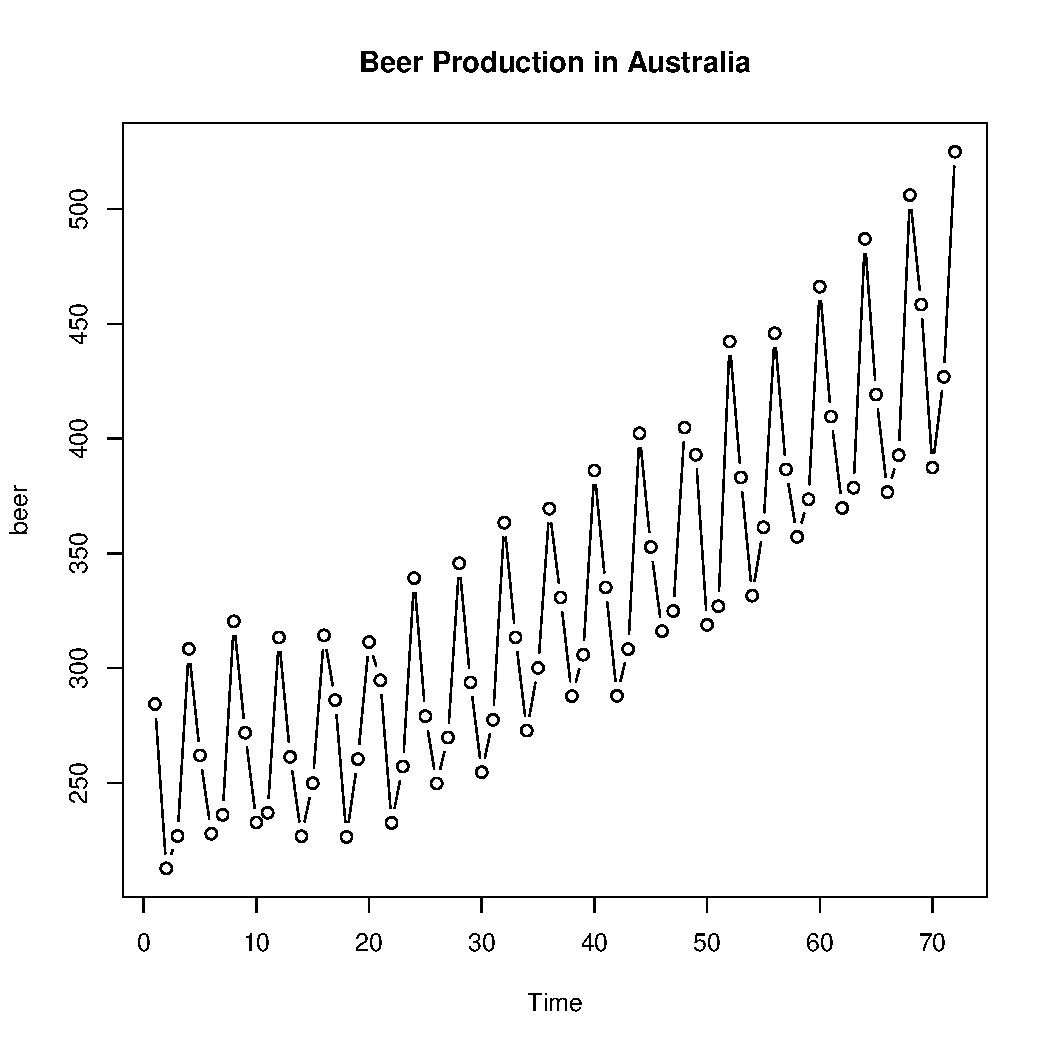
\includegraphics[width=100mm, height=60mm]{beer_ts.pdf}

\textbf{Comments on trend and/or seasonality?}

\end{frame}

\begin{frame}
\frametitle{Worked Example: Beer Production}

Based on the time series plot, we should apply both a first difference (non-seasonal) and difference with lag 4 (seasonal) to the data. Out of curiosity, we may wish to look at the time series plots of the data when just one of these differences is applied.

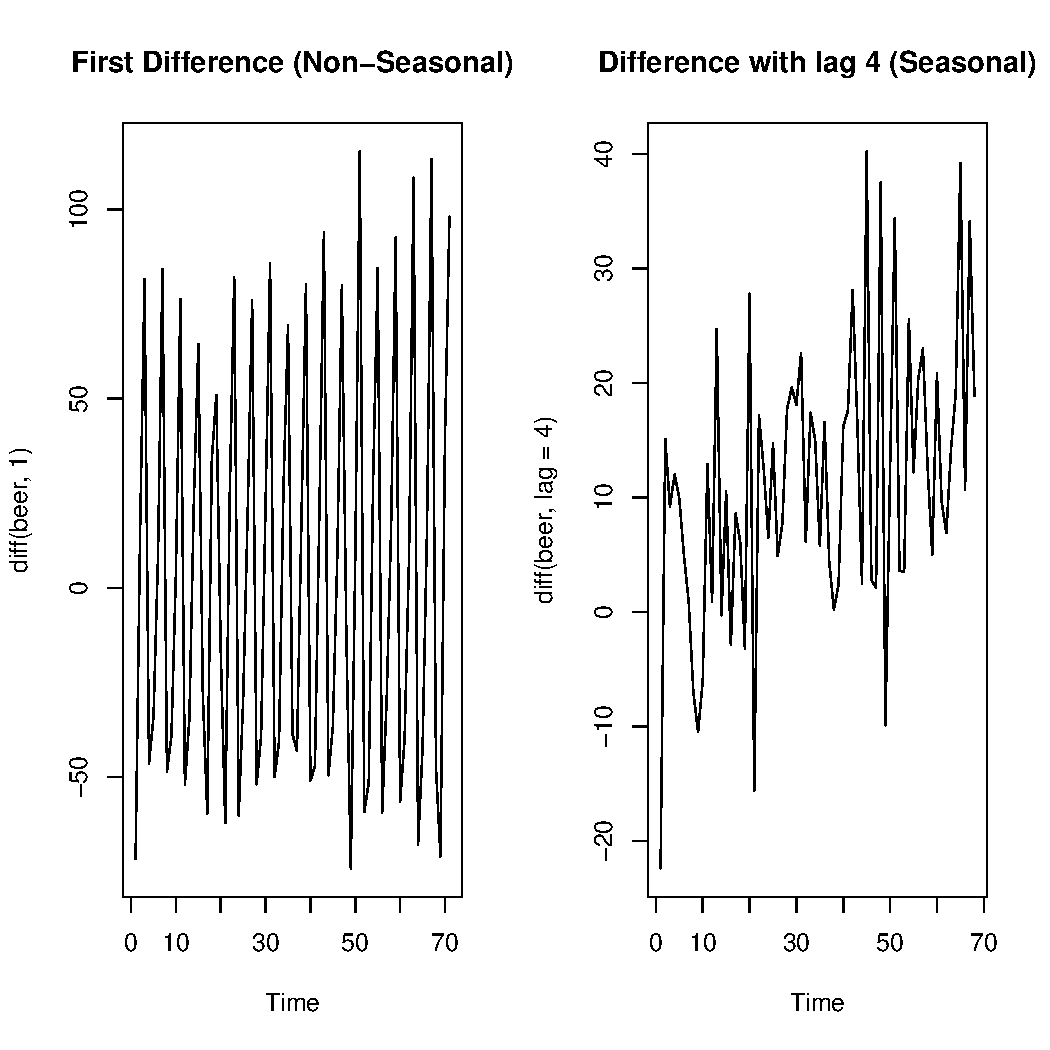
\includegraphics[width=100mm, height=50mm]{beer_tsdiff.pdf}

\textbf{Comments?}


\end{frame}

\begin{frame}
\frametitle{Worked Example: Beer Production}

Take a look at the time series of the data after both differencing operations have been applied.

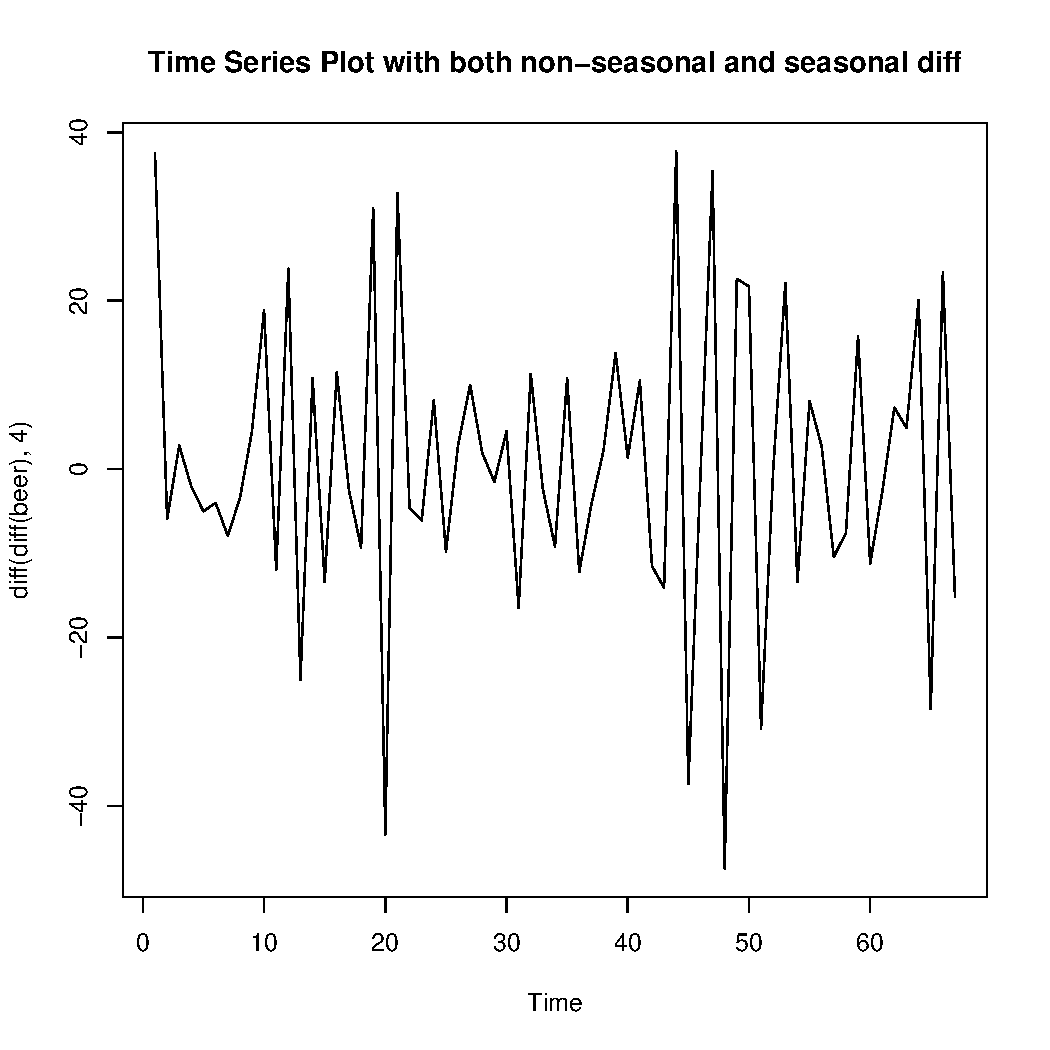
\includegraphics[width=100mm, height=60mm]{beer_tssta.pdf}

$d=1, D=1, s=4$ appear to be reasonable.


\end{frame}

\begin{frame}
\frametitle{Worked Example: Beer Production}

Examine the ACF and PACF of the data after both differencing operations.

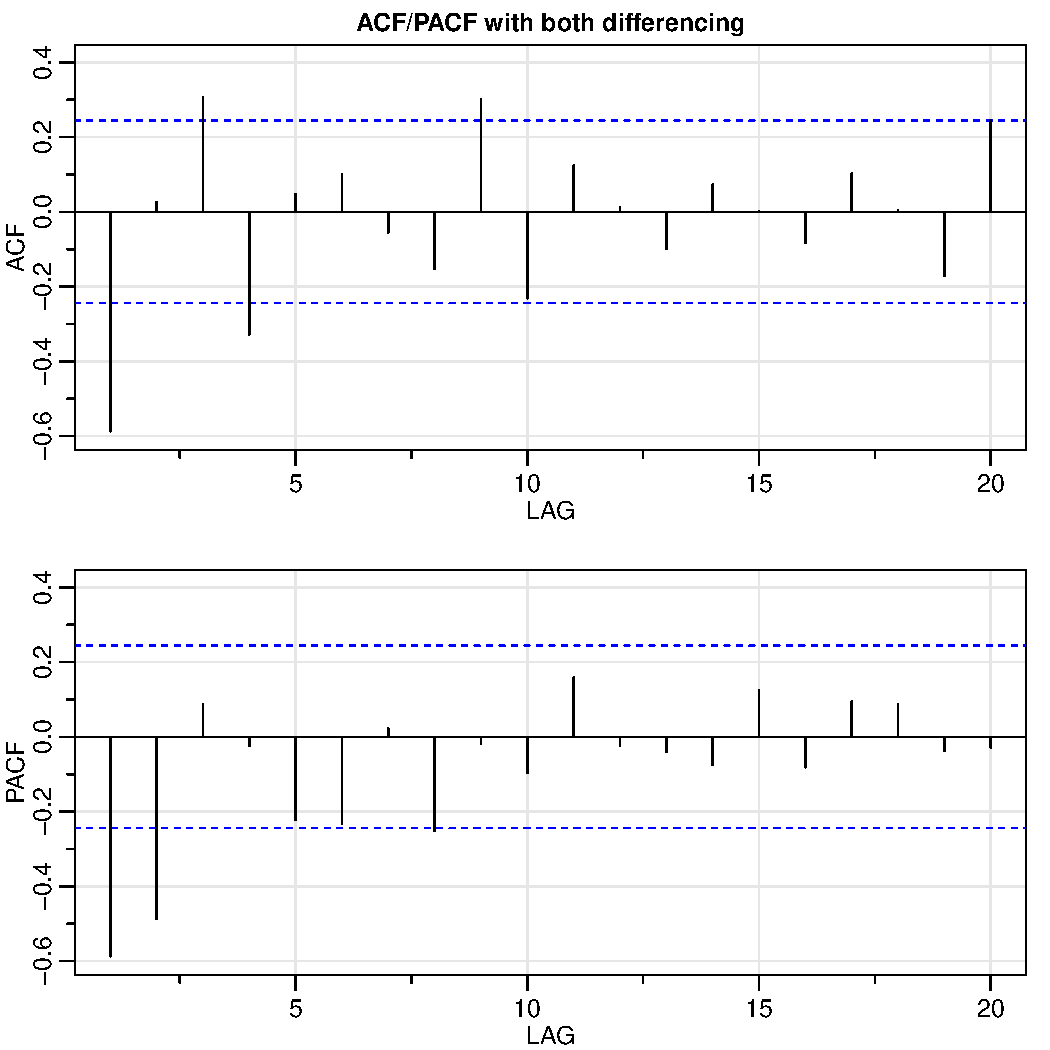
\includegraphics[width=100mm, height=60mm]{beer_acf.pdf}

\end{frame}

\begin{frame}
\frametitle{Worked Example: Beer Production}

\textbf{Question}: Thoughts on non-seasonal components, $p, q$? How about seasonal components, $P, Q$?
\end{frame}

\begin{frame}
\frametitle{Worked Example: Beer Production}

Consider the following models, based on ACF and PACF.

\begin{enumerate}
%\item ARIMA$(2,1,0) \times (0,1,1)_4$
\item ARIMA$(2,1,0) \times (0,1,1)_4$
%\item ARIMA$(0,1,1) \times (0,1,1)_4$
\item ARIMA$(0,1,1) \times (0,1,1)_4$
%\item ARIMA$(2,1,1) \times (0,1,1)_4$
\item ARIMA$(1,1,1) \times (0,1,1)_4$
\end{enumerate}

\end{frame}

\begin{frame}
\frametitle{Worked Example: Beer Production}

Model 1: ARIMA$(2,1,0) \times (0,1,1)_4$

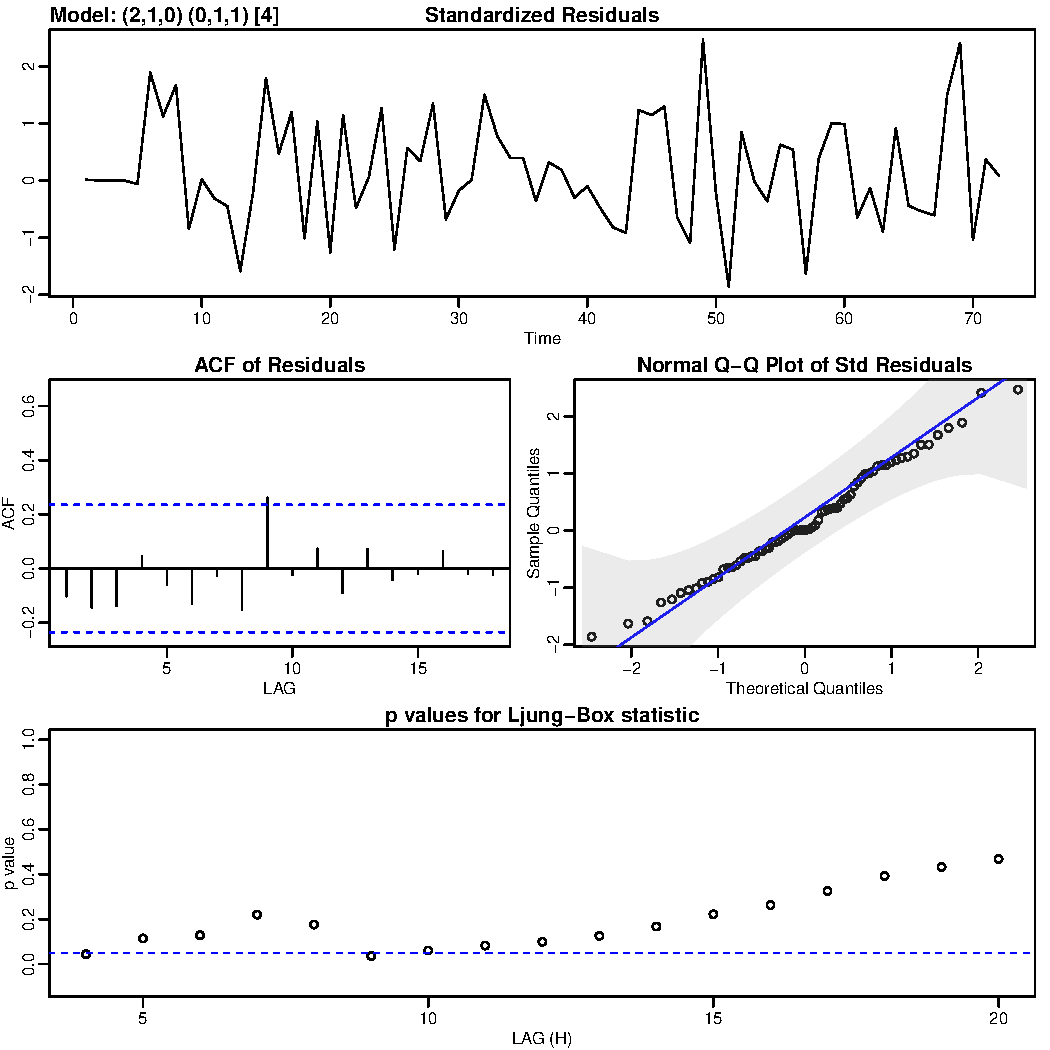
\includegraphics[width=100mm, height=60mm]{beer_m1.pdf}

\textbf{Comments?}
\end{frame}

\begin{frame}
\frametitle{Worked Example: Beer Production}

Model 2: ARIMA$(0,1,1) \times (0,1,1)_4$

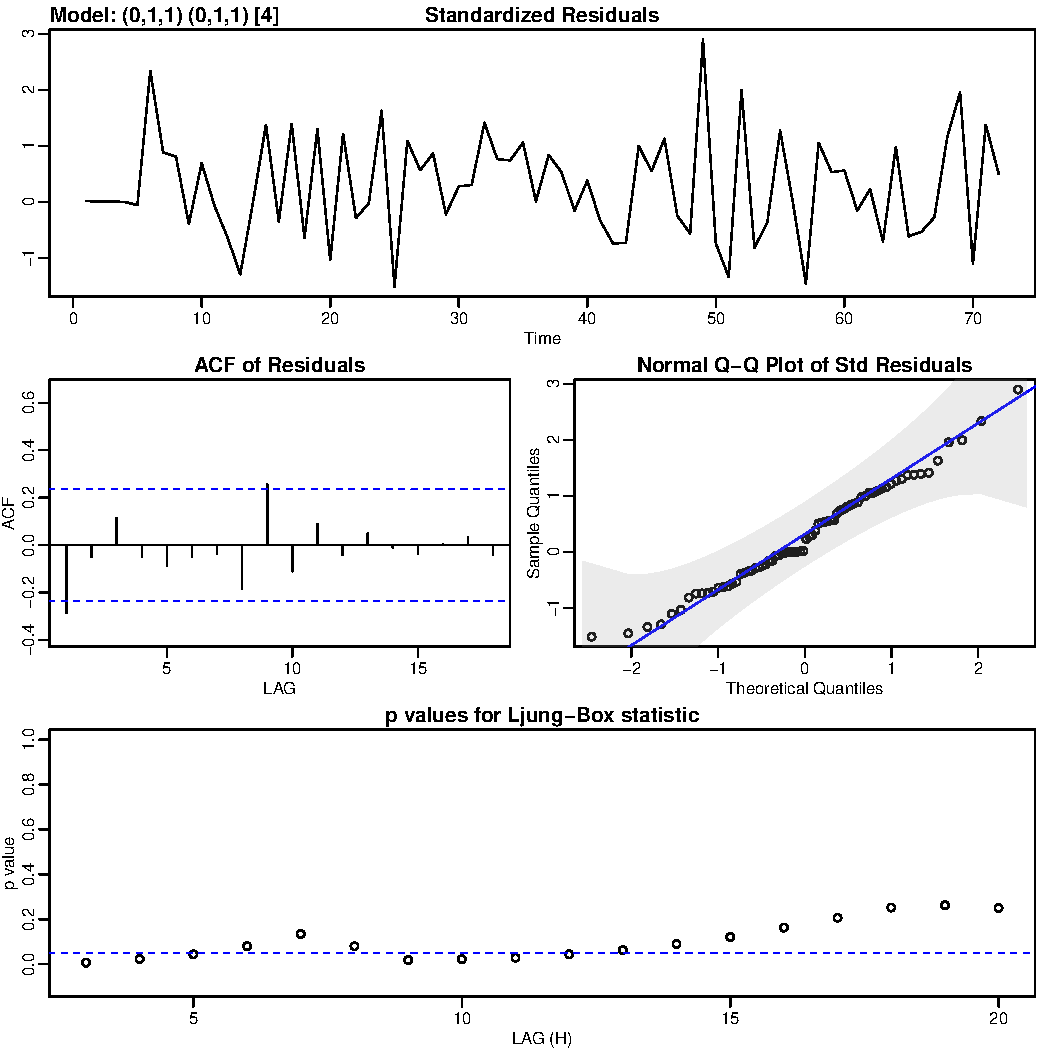
\includegraphics[width=100mm, height=60mm]{beer_m2.pdf}

\textbf{Comments?}
\end{frame}

\begin{frame}
\frametitle{Worked Example: Beer Production}

Model 3: ARIMA$(1,1,1) \times (0,1,1)_4$

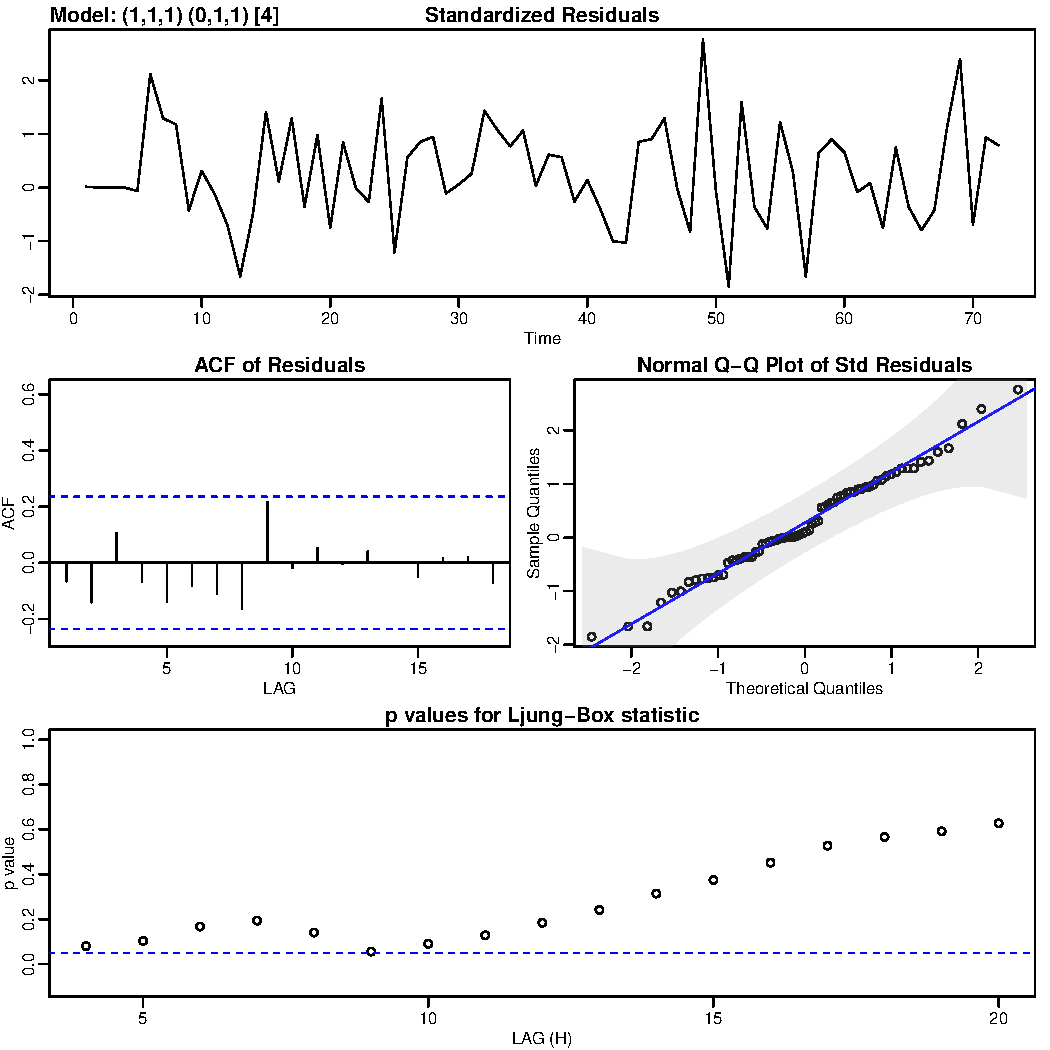
\includegraphics[width=100mm, height=60mm]{beer_m3.pdf}

\textbf{Comments?}
\end{frame}

\begin{frame}[fragile]
\frametitle{Worked Example: Beer Production}

Check the significance of the parameters for ARIMA$(1,1,1) \times (0,1,1)_4$.

\begin{verbatim}
     Estimate     SE t.value p.value
ar1   -0.3307 0.1361 -2.4289   0.018
ma1   -0.7181 0.0958 -7.4942   0.000
sma1  -0.5768 0.1165 -4.9493   0.000
\end{verbatim}

\textbf{Comments?}
\end{frame}



\end{document} 